\section{Controlled Results on TimeSage-MT}
\label{sec:probes}
TimeSage-MT provides public task records with explicit analytical procedures and deterministic downstream checks \citep{kong2026timesagemt}. Table~\ref{tab:ladder} shows the comparisons that determine the scientific interpretation. The full execution lineage, including manipulation checks and support-recovery receipts, appears in Appendix~\ref{app:probes}.

\begin{table}[t]
\centering
\small
\caption{The six comparisons that determine the paper's conclusions. ``Authority'' distinguishes a frozen score-level result from a robustness or directional result.}
\label{tab:ladder}
\begin{tabular}{@{}p{0.34\linewidth}p{0.27\linewidth}p{0.29\linewidth}@{}}
\toprule
Comparison & Paired result & Current authority \\
\midrule
Persistent targeted text vs. generic text & 11/13 vs. 10/13; $p=.500$ & no matched signal \\
Prospective supplied output vs. matched helper & 4/20 vs. 5/20; $p=.875$ & negative boundary \\
Executable Qwen vs. neutral matched helper & 6/19 vs. 2/19; $p=.109$ & directional \\
First-time STL vs. identical-interface helper & 5/7 vs. 0/7; $p=.0313$ & deterministic gate pass; semantic robustness open \\
Non-STL Qwen vs. substantive off-target procedure & 5/8 vs. 1/8; $p=.0625$ & directional; gate open \\
Non-STL DeepSeek vs. substantive off-target procedure & 5/9 vs. 2/9; $p=.125$ & directional; gate open \\
\bottomrule
\end{tabular}
\end{table}

\subsection{Weaker skill surfaces do not isolate procedure value}
Persistent text is the weakest intervention. A targeted card describes the benchmark procedure that should be retained after a misleading shortcut. Targeted succeeds on 11/13 endpoints and matched generic text succeeds on 10/13. The paired difference is +7.7 points with $p=0.50$.

Direct procedure-output injection is stronger because it places analytical results in context. A reachability check confirms that models copy numbers from the supplied output, yet the manipulation endpoint is not independent of that output. We therefore freeze 20 new tasks and score the benchmark's downstream finding. Targeted output succeeds on 4/20 tasks while the matched helper succeeds on 5/20. The paired difference is $-5.0$ points with $p=0.875$. Making the correct procedure result available in context does not establish matched downstream repair under this realization.

\subsection{Executable state produces the first matched gate pass}
The executable intervention hides the arm behind one tool surface. The target and matched arms expose the same function name. Their descriptions and argument schemas are identical. The model chooses whether to call the tool before it sees the hidden implementation result.

In the initial Qwen experiment, 19 endpoints pass pre-outcome execution qualification. Targeted succeeds on 6/19 endpoints and a content-light matched executable helper succeeds on 2/19. The paired effect is +21.1 points. Five discordant endpoints favor targeted and one favors the helper, giving exact one-sided $p=0.109375$. The preregistered +20-point magnitude criterion is met, while the full matched gate stays open. DeepSeek-v4-Pro preserves the positive direction on the same endpoints at 5/19 versus 3/19.

A separate candidate population was frozen before any later support recovery. Seven genuinely first-time recovered endpoints form an independent tranche after previously evaluated tasks are removed. Targeted succeeds on 5/7 endpoints while matched generic succeeds on 0/7. All five discordant pairs favor targeted, giving +71.4 points with exact one-sided $p=0.03125$. This passes the frozen deterministic matched gate. Every endpoint in this tranche is STL decomposition, so the formal score-level support is procedure-family specific.

We audit all 21 answers from these seven endpoints with arm labels hidden. One of the two predeclared semantic reviewers returns a complete judgment set; the other is nonvoting after a function-argument parse failure and is not replaced. The valid reviewer judges 6/7 targeted answers and 2/7 generic answers fully correct. Five pairs favor targeted and one favors generic, giving +57.1 points with exact $p=0.109375$. The semantic audit therefore does not reproduce the deterministic matched gate. It leaves the frozen score unchanged while making measurement robustness an explicit evidence debt.

The original frozen population can also be summarized after later support completion using exactly one first valid observation per executable endpoint. Twenty endpoints are available. Targeted succeeds on 10/20 and matched generic on 2/20, giving a descriptive +40.0-point effect with $p=0.00390625$. Because part of the support completion occurs after partial outcomes, this combined statistic is treated as robustness evidence and does not create a second closure test.

\subsection{A substantive off-target control tests broader procedure families}
The initial executable control performs real tool invocation while carrying little analytical content. We therefore build a new strong-control population from TimeSage-MT L2. Its 60 task IDs are frozen as a source population before any new model outcome. Fifty-eight task JSONs are available under the bounded support snapshot; two remain support debt. Measurement qualification selects the earliest non-basic target procedure whose benchmark reference output is finite and consistent with its deterministic verifier. The task must also contain an earlier substantive benchmark procedure that does not satisfy the target verifier. Twelve tasks meet the metadata rule. Nine pass execution qualification. One remains support hold and two fail reference replay or execution. No replacement task is added.

The nine qualified endpoints span five non-STL target families: time-series forest regression, residual diagnostics, linear interpolation, model comparison and ROCKET classification. The targeted tool executes the target benchmark procedure. The strong control executes the selected task-local off-target procedure. Both outputs are truncated to the same pre-frozen word count. The visible tool definition is identical across the two executable arms.

On Qwen2.5-32B, one off-target arm attempts a forbidden second tool call. The corresponding endpoint is invalid under the frozen protocol and is not retried. Eight paired endpoints remain. Targeted succeeds on 5/8 and the substantive off-target control on 1/8. The paired effect is +50.0 points. Four discordant pairs favor targeted and none favor the control, giving exact one-sided $p=0.0625$. This reaches the magnitude criterion and misses the inferential threshold by one exact step.

We repeat the exact nine-endpoint contract with DeepSeek-v4-Pro. All 27 arm records are valid. Targeted succeeds on 5/9 endpoints and the substantive off-target control succeeds on 2/9. The paired effect is +33.3 points with $p=0.125$. No-skill succeeds on 0/9, giving a secondary targeted--no-skill $p=0.03125$. Qwen and DeepSeek are adjudicated independently; their $p$-values are never pooled.

These strong-control experiments broaden the evidence beyond STL decomposition. The targeted-minus-off-target direction is positive on both model families and across five non-STL target procedures. Neither independent broad-family matched gate closes. We therefore retain broad C3 as active. The STL tranche remains the only frozen deterministic gate pass, and F11 shows that its semantic measurement robustness is not established.

\begin{figure}[t]
\centering
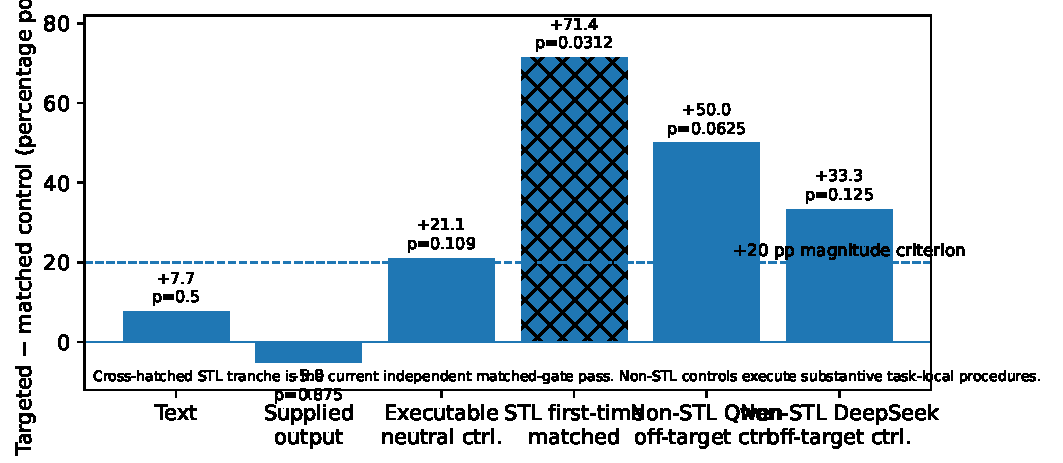
\includegraphics[width=\linewidth]{figures/fig3_independent_probes.pdf}
\caption{Matched targeted-minus-control effects for the intervention surfaces that determine the paper's conclusions. The first STL tranche passes its frozen matched gate. The non-STL strong-control experiments are directionally positive on Qwen and DeepSeek while their exact matched gates remain open.}
\label{fig:independent-probes}
\end{figure}
